\chapter{多维源代码表征学习方法总体设计}
\label{chap:design}

本章首先介绍代码表征学习面临的一些关键技术挑战,基于此提出本文的面向代码克隆检测的多维源代码表征方法框架RLCCD的研究方案,并就该框架的设计思路和总体架构进行详细阐述。此外也简要介绍了该框架包含的3个流程,即代码预处理、多维源代码表征学习、克隆检测任务实现。

\section{面向克隆检测的代码表征学习关键技术挑战}
\label{sec:challenges}

目前已有的代码克隆检测方法大多遵循以下思路:(1)首先对代码片段进行预处理;(2)对处理好的代码片段进行代码表征,将其转换为中间表征;(3)根据表征的方式不同计算不同代码片段之间的相似度,完成克隆检测任务。在代码克隆检测中,源代码表征方式决定了后续克隆检测方法的算法选择。从目前多种维度的代码表征方法来看,现有的代码表征方式存在以下技术挑战:

(1)Token维度代码表征存在集外词问题

基于Token的方法一般会将源代码表示为Token序列,然后通过词频统计,使代码文本形成一组由词频构成的数字向量,最后利用相似度计算的算法来计算两段代码的相似性。这类方法和自然语言处理(NLP)领域中常用来处理文本的方式很相似,产生一个规模巨大且稀疏的词汇表。但是,在大多数基于token的代码克隆检测工具中,通常会将token规范化,例如:将变量名用统一的标识符来代替。经过规范化的token产生的词汇表较小,导致模型学习能力有限,并且在训练过程中会出现未见过或未包含在词汇表中的词语。这些词语可能是用户自定义词、拼写错误、缩写、专有名词等。由于模型在训练阶段没有足够的信息来学习这些词语的表示,因此在实际应用中无法正确处理这些词语,从而导致模型的性能下降,这就是集外词(Out of vocabulary,简称OOV)问题。集外词问题会对模型的性能和泛化能力造成影响,严重限制了代码表征的有限性。

(2)树维度代码表征存在梯度消失问题

基于树的方法将代码转换成相应的抽象语法树,然后通过树匹配算法计算其相似度。与自然语言处理领域的长文本类似,当上下文序列很长的时候,基于树的神经网络模型容易出现梯度消失的问题,即梯度在训练过程中变得越来越小,特别是当树非常深的时候,模型会面临梯度消失问题。目前大多数基于树的代码克隆检测方法为了简化或者提高效率,通常会将生成的抽象语法树转换为完整的二叉树,在转换的过程中,不仅破坏了源代码原有的语法结构,也会增加树的高度,进一步削弱模型捕捉复杂语义的能力,导致检测性能下降。

(3)图维度代码表征存在规模开销问题

基于图的方法会将源代码表征为程序依赖图或者控制流图,然后应用图匹配算法来寻找最大的相似子图。大多数基于图的代码克隆检测工具任务的核心是将图中的每个节点映射到一个低维、稠密的特征向量中,并将这些特征编码为特征矩阵,这一步通常需要大量空间开销。同时子图匹配算法是NP完全问题,计算成本过长,时间复杂度很高,因此图维度代码表征学习会存在算法计算开销大,可扩展性不好,检测结果召回率低等问题。

(4)代码表征存在信息利用不充分问题

虽然目前代码表征在Token、树、图等多种维度的研究已经取得了一定的进展,但还存在信息利用不充分的问题。代码不仅仅具有文本自然性,同时具有结构信息、语义信息。在现有的表征粒度种,Token维度的代码表征通常只关注文本相似性,抽象语法树可以捕获程序的语法结构和模式,程序依赖图可以表达程序的部分语义信息,使用单个特征来表示代码是远远不够的,很难覆盖所有信息,因此存在信息利用不充分,特征表达不完善的问题。

\section{RLCCD框架研究方案}
\label{sec:Framework}
针对上述提出的技术中面临的关键挑战,本文提出面向代码克隆检测的多维源代码表征方法RLCCD。本节首先介绍RLCCD框架的研究思路及总体框架,然后根据流程介绍代码处理、多维源代码表征学习、克隆检测任务实现三个步骤,其中,多维源代码表征学习步骤中分别针对\ref{sec:challenges}节提出的4个关键挑战提出了对应的解决办法。

\subsection{研究思路及总体框架}
\label{subsec:Ideas}
基于上述关键技术挑战,本文提出如图所示的总体研究思路,该思路聚焦于多维源代码表征学习,通过


面向代码克隆检测的多维源代码表征学习方法RLCCD,旨在通过构建三个不同维度的代码表征模型,将源代码的语义信息表示为稠密低维实值向量,以在低维空间中高效计算实体和关系的语义联系,并通过特征融合得到多维特征,实现对代码信息的充分利用,以更加全面准确与智能化的方式提高代码克隆测试效率。 

源代码的表征方式决定了信息抽取的程度和粒度,进而影响深度学习模型的精度和效率,是代码克隆检测的基石。考虑到经由不同表征方式处理所得到的信息通常具有互补性,基于混合代码表示,通过保留多个代码特征,包括非结构化(顺序令牌形式的代码)和结构化(抽象语法树和控制流图形式的代码)信息。将多个代码特征融合成一个混合表示,该混合表示具有关注机制,该机制关注重要的代码部分和有助于最终检测准确性的特征。

多模态学习可以通过利用多模态数据之间的信息互补性,,从多源数据中学到更好的特征表示,有利于下游从多源数据中学到更好的特征表示习..因为编程语言含有多个抽象层次的特征,,所以用单个特征来表示编程语言是远远不够的,很难覆盖所有视角..并且不同的模态都是代码表示的平行语料,具有语义等价性。

本文基于上述研究思路,设计了面向代码克隆检测的多维源代码表征方法RLCCD框架,如图\ref{fig:framework}所示。由图可见,本文提出的基本框架与\ref{subsec:Code clone detection}节提出的代码克隆检测的处理流程基本一致,并主要通过三个维度对代码表征环节进行优化。

\begin{figure}[H]
    \centering
    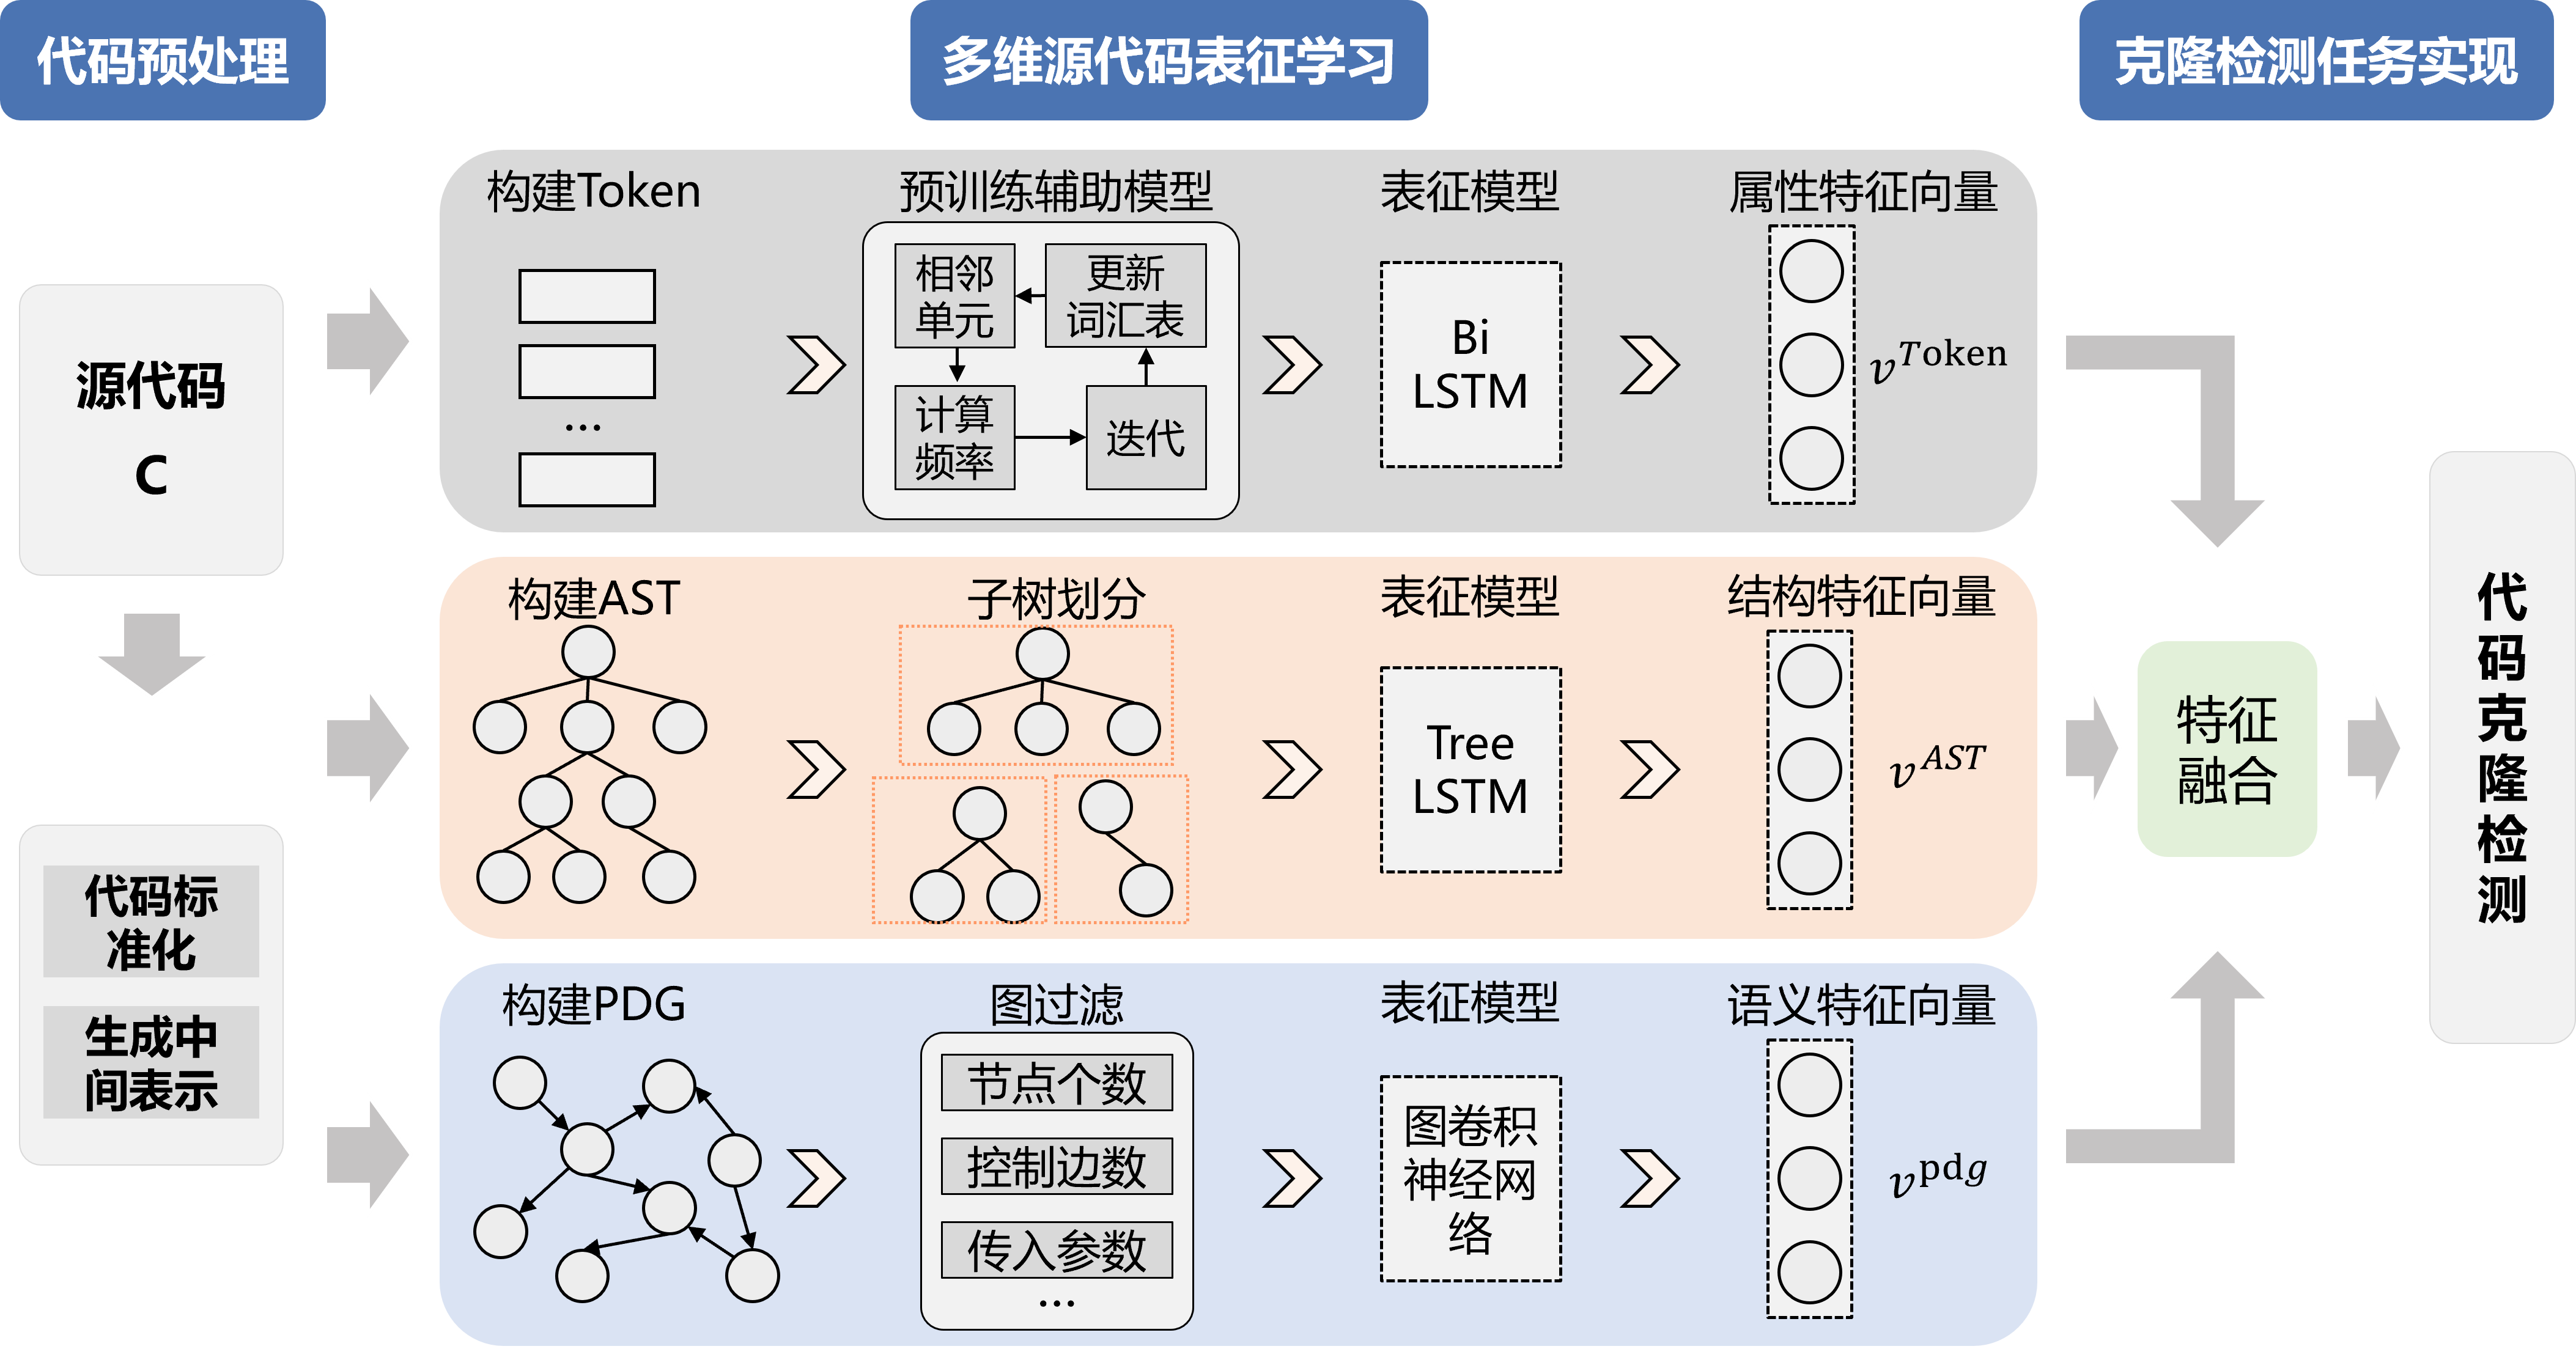
\includegraphics[width=0.95\textwidth]{figures/framework}
    \caption{RLCCD 总体框架}
    \label{fig:framework}
\end{figure}

下面则分别对代码处理、多维源代码表征学习、克隆检测任务实现的流程和关键技术点进行介绍。

\subsection{代码处理}
\label{subsec:Preprocess}
代码处理的目标是生成源代码片段对应的Token序列、抽象语法树和程序依赖图,主要包含3个流程:抽取代码块、代码标准化、生成中间表示。首先,使用TXL工具从源代码中提取出代码块。这里的源码来自POJ104公共数据基准集,而TXL是专门为软件分析和源代码转换任务设计的一个分析工具,可以很好地支持C语言;然后,对代码块中的代码进行代码标准化处理。具体的,首先需要去除代码块中的注释、空格和空行,然后根据一定的转化规则进行代码标准化;最后,基于标准化后的代码片段生成对应的中间表示:Token序列、抽象语法树AST和程序依赖图PDG。

\subsection{多维源代码表征学习}
\label{subsec:Representation}
RLCCD框架的核心步骤是源代码表征学习,其目标是学习能够表示代码片段的连续向量,表现程序理解的认知层次,获取程序的语法、语义信息,创建程序更高抽象层次上的表示,它决定着对源代码信息抽取程度的上限,决定着检测方法的预处理方式、模型设计、部署方式、运行效率,并影响后续代码克隆检测任务所能检测的精度。下面从Token序列、抽象语法树AST、程序依赖图PDG三种不同维度的代码特征表示出发,详细介绍研究方案并分析其优化改进。

(1)针对Token序列特征挖掘,提出预训练增强辅助模型提取属性特征,从而解决传统基于Token序列的方法存在的集外词问题;

(2)针对抽象语法树AST特征挖掘,提出子树划分的改进方法提取结构特征,从而解决传统基于抽象语法树的方法存在的梯度消失问题;

(3)针对程序依赖图PDG特征挖掘,提出过滤机制提取语义特征,通过收集PDG的简单特征来过滤掉明显不可能为克隆的PDG对,从而解决传统基于程序依赖图的方法存在的计算开销大问题。

(4)特征融合方法

特征融合的目标是将提取到的属性特性、结构特征、语义特征合并,得到一个更能代表代码信息的多维特征,更具有判别能力。

按照具体的技术,特征融合包括特征拼接、特征求和(均值、pooling、加权求和)、特征之间对应元素相乘、特征之间求外积再送入神经网络、跳跃连接(skip)、反卷积、典型相关分析CCA、注意力机制(包括self-attention)加权求和、构图然后采用图神经网络等等。

\subsection{克隆检测任务实现}
\label{subsec:Clone detection}
克隆检测任务实现的目标是通过计算两个代码的向量距离来判断是否存在代码克隆。常见的向量距离包括欧式距离、曼哈顿距离等。由于代码克隆检测问题是一个二分类问题,即给定两个代码片段,需要输出0或1,0表示它们之间不相似,1表示相似。因此需要将向量距离d映射到0~1之间,这里可以通过sigmoid函数、tanh函数等做映射,其函数值表示两个代码片段的相似度。然后设定阈值,当相似度大于阈值,则判定两个代码片段属于代码克隆,输出1。

\section{本章小结}
\label{sec:Summary2}
本章首先分析了源代码表征学习在代码克隆检测过程中所面临的关键技术挑战,主要表现为Token集外词问题、树梯度消失问题、图计算开销大问题。针对上述提出的三个问题,提出了本文的方法RLCCD,并介绍了其整体框架和处理流程,对其中的关键技术点进行了简要的论述。
